%% LyX 2.0.3 created this file.  For more info, see http://www.lyx.org/.
%% Do not edit unless you really know what you are doing.
\documentclass[10pt]{beamer}\usepackage[]{graphicx}\usepackage[]{color}
%% maxwidth is the original width if it is less than linewidth
%% otherwise use linewidth (to make sure the graphics do not exceed the margin)
\makeatletter
\def\maxwidth{ %
  \ifdim\Gin@nat@width>\linewidth
    \linewidth
  \else
    \Gin@nat@width
  \fi
}
\makeatother

\definecolor{fgcolor}{rgb}{0.345, 0.345, 0.345}
\newcommand{\hlnum}[1]{\textcolor[rgb]{0.686,0.059,0.569}{#1}}%
\newcommand{\hlstr}[1]{\textcolor[rgb]{0.192,0.494,0.8}{#1}}%
\newcommand{\hlcom}[1]{\textcolor[rgb]{0.678,0.584,0.686}{\textit{#1}}}%
\newcommand{\hlopt}[1]{\textcolor[rgb]{0,0,0}{#1}}%
\newcommand{\hlstd}[1]{\textcolor[rgb]{0.345,0.345,0.345}{#1}}%
\newcommand{\hlkwa}[1]{\textcolor[rgb]{0.161,0.373,0.58}{\textbf{#1}}}%
\newcommand{\hlkwb}[1]{\textcolor[rgb]{0.69,0.353,0.396}{#1}}%
\newcommand{\hlkwc}[1]{\textcolor[rgb]{0.333,0.667,0.333}{#1}}%
\newcommand{\hlkwd}[1]{\textcolor[rgb]{0.737,0.353,0.396}{\textbf{#1}}}%
\newcommand\myeq{\stackrel{\mathclap{\normalfont\mbox{d}}}{=}}




\usepackage{fontawesome5}
\usepackage{framed}
\makeatletter
\newenvironment{kframe}{%
 \def\at@end@of@kframe{}%
 \ifinner\ifhmode%
  \def\at@end@of@kframe{\end{minipage}}%
  \begin{minipage}{\columnwidth}%
 \fi\fi%
 \def\FrameCommand##1{\hskip\@totalleftmargin \hskip-\fboxsep
 \colorbox{shadecolor}{##1}\hskip-\fboxsep
     % There is no \\@totalrightmargin, so:
     \hskip-\linewidth \hskip-\@totalleftmargin \hskip\columnwidth}%
 \MakeFramed {\advance\hsize-\width
   \@totalleftmargin\z@ \linewidth\hsize
   \@setminipage}}%
 {\par\unskip\endMakeFramed%
 \at@end@of@kframe}
\makeatother

\definecolor{shadecolor}{rgb}{.97, .97, .97}
\definecolor{messagecolor}{rgb}{0, 0, 0}
\definecolor{warningcolor}{rgb}{1, 0, 1}
\definecolor{errorcolor}{rgb}{1, 0, 0}
\newenvironment{knitrout}{}{} % an empty environment to be redefined in TeX

\usepackage{alltt}
\usepackage[T1]{fontenc}
\setcounter{secnumdepth}{3}
\setcounter{tocdepth}{3}
\usepackage{tikz}
\usepackage{color}
\usepackage{colortbl}
\usepackage{dcolumn}
\usepackage{amsmath}
\usepackage{tikz}
\usepackage{floatflt}
\usepackage{multicol}
\usepackage{multirow}
\usepackage{listings}
\usepackage{tabularx}
\usepackage{amssymb}% http://ctan.org/pkg/amssymb
\usepackage{pifont}% http://ctan.org/pkg/pifont
\usepackage{bbm}
\usepackage{siunitx}
\usepackage{url}
\usepackage{verbatim}
\usepackage{enumerate}
\usepackage{algorithmic}
\usepackage{algorithm}
\usepackage[flushleft]{threeparttable}
\usepackage{algorithm}
\usepackage{amsfonts}
\usepackage{booktabs}
\usepackage{siunitx}

\usepackage{hyperref}
\hypersetup{
    colorlinks=magenta,
    linkcolor=blue,
    filecolor=magenta,      
    urlcolor=magenta
     }
     
    \definecolor{links}{HTML}{2A1B81}
\hypersetup{colorlinks,linkcolor=blue, urlcolor=magenta}


\makeatletter

%%%%%%%%%%%%%%%%%%%%%%%%%%%%%% LyX specific LaTeX commands.
\providecommand{\LyX}{\texorpdfstring%
  {L\kern-.1667em\lower.25em\hbox{Y}\kern-.125emX\@}
  {LyX}}


%%%%%%%%%%%%%%%%%%%%%%%%%%%%%% Textclass specific LaTeX commands.
 % this default might be overridden by plain title style
 \newcommand\makebeamertitle{\frame{\maketitle}}%
 \AtBeginDocument{
   \let\origtableofcontents=\tableofcontents
   \def\tableofcontents{\@ifnextchar[{\origtableofcontents}{\gobbletableofcontents}}
   \def\gobbletableofcontents#1{\origtableofcontents}
 }
 \def\lyxframeend{} % In case there is a superfluous frame end
 \long\def\lyxframe#1{\@lyxframe#1\@lyxframestop}%
 \def\@lyxframe{\@ifnextchar<{\@@lyxframe}{\@@lyxframe<*>}}%
 \def\@@lyxframe<#1>{\@ifnextchar[{\@@@lyxframe<#1>}{\@@@lyxframe<#1>[]}}
 \def\@@@lyxframe<#1>[{\@ifnextchar<{\@@@@@lyxframe<#1>[}{\@@@@lyxframe<#1>[<*>][}}
 \def\@@@@@lyxframe<#1>[#2]{\@ifnextchar[{\@@@@lyxframe<#1>[#2]}{\@@@@lyxframe<#1>[#2][]}}
 \long\def\@@@@lyxframe<#1>[#2][#3]#4\@lyxframestop#5\lyxframeend{%
   \frame<#1>[#2][#3]{\frametitle{#4}#5}}

\renewcommand{\footnotesize}{\fontsize{6pt}{6pt}\selectfont}


\newcommand{\indep}{\rotatebox[origin=c]{90}{$\models$}}

% https://dkumor.com/posts/technical/2018/08/15/causal-tikz/

% Tikz settings optimized for causal graphs.
% Just copy-paste this part
\usetikzlibrary{shapes,decorations,arrows,calc,arrows.meta,fit,positioning}
\tikzset{
    -Latex,auto,node distance =1 cm and 1 cm,semithick,
    state/.style ={ellipse, draw, minimum width = 0.7 cm},
    point/.style = {circle, draw, inner sep=0.04cm,fill,node contents={}},
    bidirected/.style={Latex-Latex,dashed},
    el/.style = {inner sep=2pt, align=left, sloped}
}


%%%%%%%%%%%%%%%%%%%%%%%%%%%%%% User specified LaTeX commands.
%\usetheme{Warsaw}
\usetheme{Boadilla}
%\setbeamertemplate{navigation symbols}{}
%gets rid of bottom navigation bars
%\setbeamertemplate{footline}[page number]{}
%\setcounter{page}{44}
%\setbeamertemplate{footline}{}


\makeatother
\IfFileExists{upquote.sty}{\usepackage{upquote}}{}

\begin{document}


\title[Deconstructing Data Science Questions]{Deconstructing Data Science Questions}
\subtitle{A Case Study on Personalization}
\author[Leo Guelman]{Leo Guelman}
\institute[RBC Royal Bank]{RBC Royal Bank}
\date[December 2022]
{}
\makebeamertitle

\lyxframeend{}


%%%%Slide

%%%%Slide

\begin{frame}
[fragile]\frametitle{Talk Overview}



\begin{itemize}

\item The practice of Data Science often places significant focus on adopting sound technical methods.

\item However, much less effort is often placed on business problem identification.

\item Using Personalized Marketing problem as a motivating example:

\begin{itemize}

\item Show (fiction) story on how 4 different Data Scientists might approach this problem and get different conclusions from data.

\item Show that the different conclusions emerge as a result of slightly different interpretation of the business question being asked.

\end{itemize}

\end{itemize}


\end{frame}


%%%%Slide

\begin{frame}
[fragile]\frametitle{The Business Setting}

\begin{itemize}

\item \textbf{Business Objective:} Cross-sell a credit card to new-to-RBC clients. 


\item \textbf{Offer/Incentive:}


\begin{figure}
   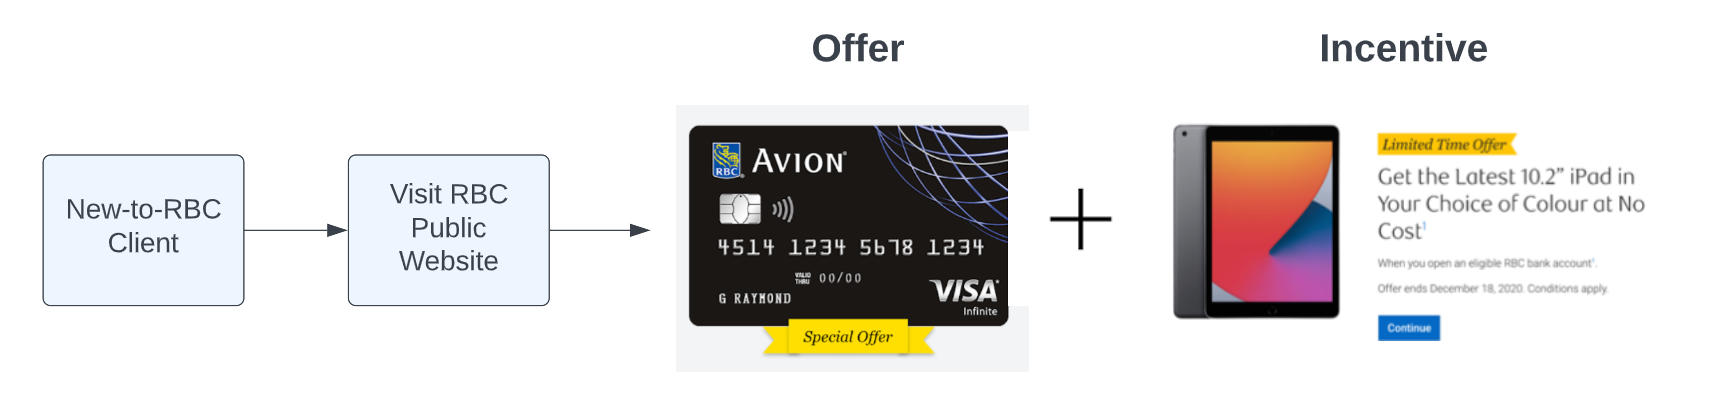
\includegraphics[width= 0.80\linewidth]{figures/campaign.png}
\end{figure}

\vskip20pt

\item \textbf{Goal:} Maximize the expected profitability of the campaign on the new-to-RBC client segment. 

%Identify which new-to-RBC clients should receive an iPad incentive in the future to maximize the expected profitability of the campaign. 

\end{itemize}

\end{frame}

%%%%Slide

\begin{frame}
[fragile]\frametitle{Data Generating Process}


\begin{columns}[T] % align columns
\begin{column}{.48\textwidth}

\begin{figure}
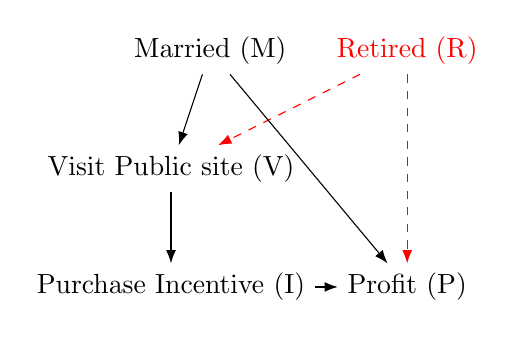
\begin{tikzpicture}
    \node (m) at (-0.5,0) {Married (M)};
    \node[red]  (r) at (2,0) {Retired (R)};
    \node (v) at (-1,-1.5) {Visit Public site (V)};
    \node (o) at (-1,-3) {Purchase Incentive (I)};
    \node (p) at (2,-3) {Profit (P)};

    \path (m) edge (v);
    \path[dashed, red] (r) edge (v);
     \path (m) edge (p);
     \path[dashed, red] (r) edge (p);
     \path (v) edge (o);
     \path (o) edge (p);
     
\end{tikzpicture}

\vskip 5pt

\caption{Causal DAG}

\end{figure}

\end{column}%
\hfill%

\pause

\begin{column}{.48\textwidth}

\vskip 20pt

\begin{equation*}
\begin{align*}
V :=& M~$\oplus{}$ R  \\
I :=&  V \\
\end{align*}
\end{equation*}
%}

\footnotesize{
\begin{table}
\begin{tabular}{ccccc}
\toprule
 &\multicolumn{2}{c}{$R=0$}
&
\multicolumn{2}{c}{$R=1$} \\\cmidrule(r){2-3}\cmidrule(l){4-5}
 & $M=1$ & $M=0$     & $M=1$ & $M=0$     \\  
 \midrule
$I=1$ &  \cellcolor{blue!25}{0.25} & 0.50 & 0.45 & \cellcolor{blue!25}{0.05} \\
$I=0$ &  0.50 & \cellcolor{blue!25}{0.10} & \cellcolor{blue!25}{0.05} & 0.30 \\
\bottomrule
\end{tabular}
\vskip5pt
\caption{$E[P|M, R, I]$. Highlighted cells reflect (new-to-RBC) client's 'natural' choice to visit the Public site or not.}
\end{table}
}


\end{column}%
\end{columns}
\end{frame}

%%%%Slide

\begin{frame}
[fragile]\frametitle{Data Scientist 1: Empirical Decision Criterion (EDC)}

\begin{columns}[T] % align columns
\begin{column}{.48\textwidth}

\begin{center}
EDC  $\rightarrow$ $\underset{I \in {0,1}}{\mathrm{argmax}}~E[P|I, M]$
\end{center}

\vskip10pt


\begin{equation*}
\begin{align*}
E[P | I=1, M=1] = 0.25\\
E[P | I=0, M=1] = 0.05\\
E[P | I=1, M=0] = 0.05\\
E[P | I=0, M=0] = 0.10\\
\end{align*}
\end{equation*}


\end{column}%
\hfill%


\begin{column}{.48\textwidth}

\footnotesize{
\begin{table}
 \begin{tabular}{ccccc}
\toprule
 &\multicolumn{2}{c}{$R=0$}
&
\multicolumn{2}{c}{$R=1$} \\\cmidrule(r){2-3}\cmidrule(l){4-5}
 & $M=1$ & $M=0$     & $M=1$ & $M=0$     \\  
 \midrule
$I=1$ &  \cellcolor{blue!25}{0.25} & 0.50 & 0.45 & \cellcolor{blue!25}{0.05} \\
$I=0$ &  0.50 & \cellcolor{blue!25}{0.10} & \cellcolor{blue!25}{0.05} & 0.30 \\
\bottomrule
\end{tabular}
\vskip5pt
\caption{$E[P|M, R, I]$.}
\end{table}
}



\end{column}%
\end{columns}

\vskip15pt


\textbf{Decision Rule}:

\small{
\begin{itemize}
\item If Visit Site $\land$ Married $\rightarrow$ Purchase Incentive $\rightarrow~E[P] = \textbf{0.25}  $
\item If Visit Site $\land$ Not Married $\rightarrow$ No Purchase Incentive  $\rightarrow~E[P] = \textbf{0.05} $
\end{itemize}
}

\vskip10pt

Expected profit = $\boxed{\mathbf{0.15}}$ = (0.25+0.05)/2.



\end{frame}


%%%%Slide

\begin{frame}
[fragile]\frametitle{Data Scientist 2: Post-Visit Randomization (PVR)}

\begin{columns}[T] % align columns
\begin{column}{.48\textwidth}

\begin{figure}
\begin{tikzpicture}[thick,scale=0.8, every node/.style={scale=0.8}]
    \node (m) at (-0.5,0) {Married (M)};
    \node[red]  (r) at (2,0) {Retired (R)};
    \node (v) at (-1,-1.5) {Visit Public site (V)};
    \node (o) at (-1,-3) {Purchase Incentive (I)};
    \node (p) at (2,-3) {Profit (P)};
    \node[blue] (c)  at (-4,-1.5) {Coin Flip (C)};

    \path (m) edge (v);
    \path[dashed, red] (r) edge (v);
     \path (m) edge (p);
     \path[dashed, red] (r) edge (p);
     \path (v) edge (o);
     \path (o) edge (p);
     \path[blue] (c) edge (o)
     
\end{tikzpicture}

\vskip 5pt

\caption{Causal DAG with post-visit randomization.}

\end{figure}

\end{column}%

\begin{column}{.48\textwidth}


\vskip 20pt

\begin{equation*}
\begin{align*}
V :=& M~$\oplus{}$ R  \\
I :=&  V \textcolor{blue}{\land C} \\
\end{align*}
\end{equation*}
%}

\end{column}%
\end{columns}

\end{frame}


%%%%Slide

\begin{frame}
[fragile]\frametitle{Data Scientist 2: Post-Visit Randomization (PVR) - cont'd}


\begin{columns}[T] % align columns
\begin{column}{.48\textwidth}

\begin{center}
PVR $\rightarrow$ $\underset{I \in {0,1}}{\mathrm{argmax}}~E[P| do(I), M, V=1]$
\end{center}

\vskip10pt


\begin{equation*}
\begin{align*}
E[P | do(I=1), M=1, V=1] = 0.25\\
E[P | do(I=0), M=1, V=1] = 0.50\\
E[P | do(I=1), M=0, V=1] = 0.05\\
E[P | do(I=0), M=0, V=1] = 0.30\\
\end{align*}
\end{equation*}


\end{column}%
\hfill%


\begin{column}{.48\textwidth}

\footnotesize{
\begin{table}
 \begin{tabular}{ccccc}
\toprule
 &\multicolumn{2}{c}{$R=0$}
&
\multicolumn{2}{c}{$R=1$} \\\cmidrule(r){2-3}\cmidrule(l){4-5}
 & $M=1$ & $M=0$     & $M=1$ & $M=0$     \\  
 \midrule
$I=1$ &  \cellcolor{blue!25}{0.25} & 0.50 & 0.45 & \cellcolor{blue!25}{0.05} \\
$I=0$ &  0.50 & \cellcolor{blue!25}{0.10} & \cellcolor{blue!25}{0.05} & 0.30 \\
\bottomrule
\end{tabular}
\vskip5pt
\caption{$E[P|M, R, I]$.}
\end{table}
}



\end{column}%
\end{columns}

\vskip15pt


\textbf{Decision Rule}:

\small{
\begin{itemize}
\item If Visit Site $\land$ Married $\rightarrow$ No Purchase Incentive $\rightarrow~E[P] = \textbf{0.50} $
\item If Visit Site $\land$ Not Married $\rightarrow$ No Purchase Incentive  $\rightarrow~E[P] = \textbf{0.30} $
\end{itemize}
}

\vskip10pt

Expected profit = $\boxed{\mathbf{0.40}}$ = (0.50+0.30)/2.



\end{frame}

%%%%Slide


\begin{frame}
[fragile]\frametitle{Data Scientist 3: RCT on New-to-RBC Clients}

\begin{columns}[T] % align columns
\begin{column}{.48\textwidth}

\begin{figure}
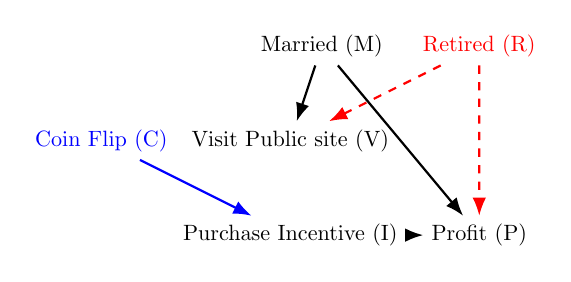
\begin{tikzpicture}[thick,scale=0.8, every node/.style={scale=0.8}]
    \node (m) at (-0.5,0) {Married (M)};
    \node[red]  (r) at (2,0) {Retired (R)};
    \node (v) at (-1,-1.5) {Visit Public site (V)};
    \node (o) at (-1,-3) {Purchase Incentive (I)};
    \node (p) at (2,-3) {Profit (P)};
    \node[blue] (c)  at (-4,-1.5) {Coin Flip (C)};

    \path (m) edge (v);
    \path[dashed, red] (r) edge (v);
     \path (m) edge (p);
     \path[dashed, red] (r) edge (p);
     \path (o) edge (p);
     \path[blue] (c) edge (o);
     
\end{tikzpicture}

\vskip 5pt

\caption{Causal DAG with RCT.}

\end{figure}

\end{column}%

\begin{column}{.48\textwidth}


\vskip 20pt

\begin{equation*}
\begin{align*}
V :=& M~$\oplus{}$ R  \\
I :=&  \textcolor{blue}{C} \\
\end{align*}
\end{equation*}
%}

\end{column}%
\end{columns}




\end{frame}

%%%%Slide


\begin{frame}
[fragile]\frametitle{Data Scientist 3: RCT on New-to-RBC Clients - cont'd}

\begin{columns}[T] % align columns
\begin{column}{.48\textwidth}

\begin{center}
RCT  $\rightarrow$ $\underset{I \in {0,1}}{\mathrm{argmax}}~E[P|do(I), M]$
\end{center}

\vskip10pt

\scriptsize{
\begin{equation*}
\begin{align*}
E[P | do(I=1), M=1] &= 0.350 =(0.25+0.45)/2 \\
E[P | do(I=0), M=1] &= 0.275 =(0.50 + 0.05)/2 \\
E[P | do(I=1), M=0] &= 0.275 =(0.50 + 0.05)/2 \\
E[P | do(I=0), M=0] &= 0.200 = (0.10 +0.30)/2 \\
\end{align*}
\end{equation*}
}


\end{column}%
\hfill%


\begin{column}{.48\textwidth}

\vskip30pt

\footnotesize{
\begin{table}
 \begin{tabular}{ccccc}
\toprule
 &\multicolumn{2}{c}{$R=0$}
&
\multicolumn{2}{c}{$R=1$} \\\cmidrule(r){2-3}\cmidrule(l){4-5}
 & $M=1$ & $M=0$     & $M=1$ & $M=0$     \\  
 \midrule
$I=1$ &  \cellcolor{blue!25}{0.25} & 0.50 & 0.45 & \cellcolor{blue!25}{0.05} \\
$I=0$ &  0.50 & \cellcolor{blue!25}{0.10} & \cellcolor{blue!25}{0.05} & 0.30 \\
\bottomrule
\end{tabular}
\vskip5pt
\caption{$E[P|M, R, I]$.}
\end{table}
}



\end{column}%
\end{columns}

\vskip15pt


\textbf{Decision Rule}:

\small{
\begin{itemize}
\item If  Married $\rightarrow$ Purchase Incentive $\rightarrow~E[P] = \textbf{0.35}  $
\item If  Not Married $\rightarrow$ Purchase Incentive  $\rightarrow~E[P] = \textbf{0.275} $
\end{itemize}
}

\vskip10pt

Expected profit = $\boxed{\mathbf{0.315}}$ = (0.35+0.275)/2.

\end{frame}

%%%%Slide

\begin{frame}
[fragile]\frametitle{Data Scientist 4: Regret Decision Criterion (RDC)}

RDC  $\rightarrow$ $\underset{a' \in~{0,1}}{\mathrm{argmax}}~E[P_{a'}| I=a, M]$

\vskip10pt

\pause

\scriptsize{
\begin{equation*}
\begin{align*}
P(\pi_{a'}, M) &= P(\pi_{a'}, M, a') +  P(\pi_{a'}, M, a) \\
                      &=  P(\pi_{a'} | M, a') P(M, a') + P(\pi_{a'} | M, a) P(M, a) \\ \\
 P(\pi_{a'} | M)  &= P(\pi_{a'} | M, a') P( a' | M)  + P(\pi_{a'} | M, a) P(a | M) \\
                        &= P(\pi | M, a') P( a' | M)  + P(\pi_{a'} | M, a) P(a | M) ~\text{(from Consistency)} \\ \\
P(\pi_{a'} | M, a) &= \frac{1}{P(a|M)} \Bigl[P(\pi_{a'} | M) -  P(\pi | M, a') P( a' | M) \Bigr] \\
&= \boxed{\frac{1}{P(a|M)} \Bigl[P\Big(\pi | M, do(a')\Big) -  P(\pi | M, a') P( a' | M) \Bigr]}\\
\end{align*}
\end{equation*}
}

\end{frame}

%%%%Slide

\begin{frame}
[fragile]\frametitle{Data Scientist 4: Regret Decision Criterion (RDC) - cont'd}

\begin{columns}[T] % align columns
\begin{column}{.48\textwidth}


\begin{scriptsize}
$\boxed{P(\pi_{I=1} | M=1, I=0)} = $
\begin{equation*}
\begin{flalign*}
 \frac{1}{P(I=0|M=1)} \Bigl[P\Big(\pi | M=1, do(I=1)\Big) -  \\
 P(\pi | M=1, I=1) P( I=1 | M=1) \Bigr].  & \\
  \frac{1}{1/2} (0.350-0.25  \times \frac{1}{1/2})  & = \textbf{0.45}
\end{flalign*}
\end{equation*}

$\boxed{P(\pi_{I=1} | M=0, I=0)} = \textbf{0.50} \\ $ 

$\boxed{P(\pi_{I=0} | M=1, I=1)} = \textbf{0.50} \\ $ 

$\boxed{P(\pi_{I=0} | M=0, I=1)} = \textbf{0.30} \\ $ 

\end{scriptsize}


\end{column}%
\hfill%


\begin{column}{.48\textwidth}

\footnotesize{
\begin{table}
 \begin{tabular}{ccccc}
\toprule
 &\multicolumn{2}{c}{$R=0$}
&
\multicolumn{2}{c}{$R=1$} \\\cmidrule(r){2-3}\cmidrule(l){4-5}
 & $M=1$ & $M=0$     & $M=1$ & $M=0$     \\  
 \midrule
$I=1$ &  \cellcolor{blue!25}{0.25} & 0.50 & 0.45 & \cellcolor{blue!25}{0.05} \\
$I=0$ &  0.50 & \cellcolor{blue!25}{0.10} & \cellcolor{blue!25}{0.05} & 0.30 \\
\bottomrule
\end{tabular}
\vskip5pt
\caption{$E[P|M, R, I]$.}
\end{table}
}

\end{column}%
\end{columns}

\vskip5pt

\scriptsize{
\textbf{Decision Rule}:

\small{
\begin{itemize}
\item If Visit Site $\land$ Married $\rightarrow$ No Purchase Incentive $\rightarrow~E[P] = \textbf{0.50} $
\item If Visit Site $\land$ Not Married $\rightarrow$ No Purchase Incentive  $\rightarrow~E[P] = \textbf{0.30} $
\item If Not Visit Site $\land$ Married $\rightarrow$ Purchase Incentive $\rightarrow~E[P] = \textbf{0.45} $
\item If Not Visit Site $\land$ Not Married $\rightarrow$ Purchase Incentive  $\rightarrow~E[P] = \textbf{0.50} $
\end{itemize}
}


\vskip5pt

Expected profit = $\boxed{\mathbf{0.4375}}$ = (0.50 + 0.30+ .45+0.50)/4.
}

\end{frame}

%%%%Slide

\begin{frame}
[fragile]\frametitle{Summary}

\begin{itemize}
\item Summarize results so far from the various criteria and emphasize no result is right or wrong, they answer different questions, but some questions are more preferable than others in specific context. 

\item Compare to oracle


\item Profit =0.4375

\end{itemize}


\end{frame}

%%%%Slide

\begin{frame}
[fragile]\frametitle{Extensions}

\begin{itemize}

\item Multiple Actions

\item Online policy optimization (e.g., MABUC)

\end{itemize}

\end{frame}

%%%%Slide

\begin{frame}
[fragile]\frametitle{The Personalization Paradigm}

\begin{itemize}

\item Illustration that shows that what is good for person 1 might be neutral or even harmful for person 2. 

\item Motivating illustration in healthcare, marketing, client-level decision making. 

\end{itemize}
  
\end{frame}



%%%%Slide

\begin{frame}
[fragile]\frametitle{Notes}

For each Data Science articulate what is the question being asked!!!!!

The conclusion should be that although DS 4 achieves highest reward, wether that is the right solution, depends on the question being asked. 


\end{frame}

\end{document}

